% ---------------------------------------------------------------
% Generated by FlowTikZ (flowcharts and data charts to LaTeX)
% Every coordinate below is derived from the editor diagram model.
% Safe to edit by hand, but regenerating will overwrite changes.
% ---------------------------------------------------------------

\documentclass[border=8pt]{standalone}
\usepackage[T1]{fontenc}
\usepackage[utf8]{inputenc}
\usepackage{amsmath}
\usepackage{amssymb}
\usepackage{xcolor}
\usepackage{tikz}

% ---- Colour definitions ----
\definecolor{fc12161C}{HTML}{12161C}

% ---- Style definitions ----
\tikzset{
  fcnode/.style={
    draw, inner sep=0pt, outer sep=0pt, align=center,
    line join=round, line cap=butt
  },
  fcpath/.style={line join=round, line cap=butt},
  fcedge/.style={line join=round, line cap=butt},
  fclabel/.style={inner sep=1.4pt, outer sep=0pt, align=center},
}
\tikzset{fcformula/.style={inner sep=0pt, outer sep=0pt}}

\begin{document}
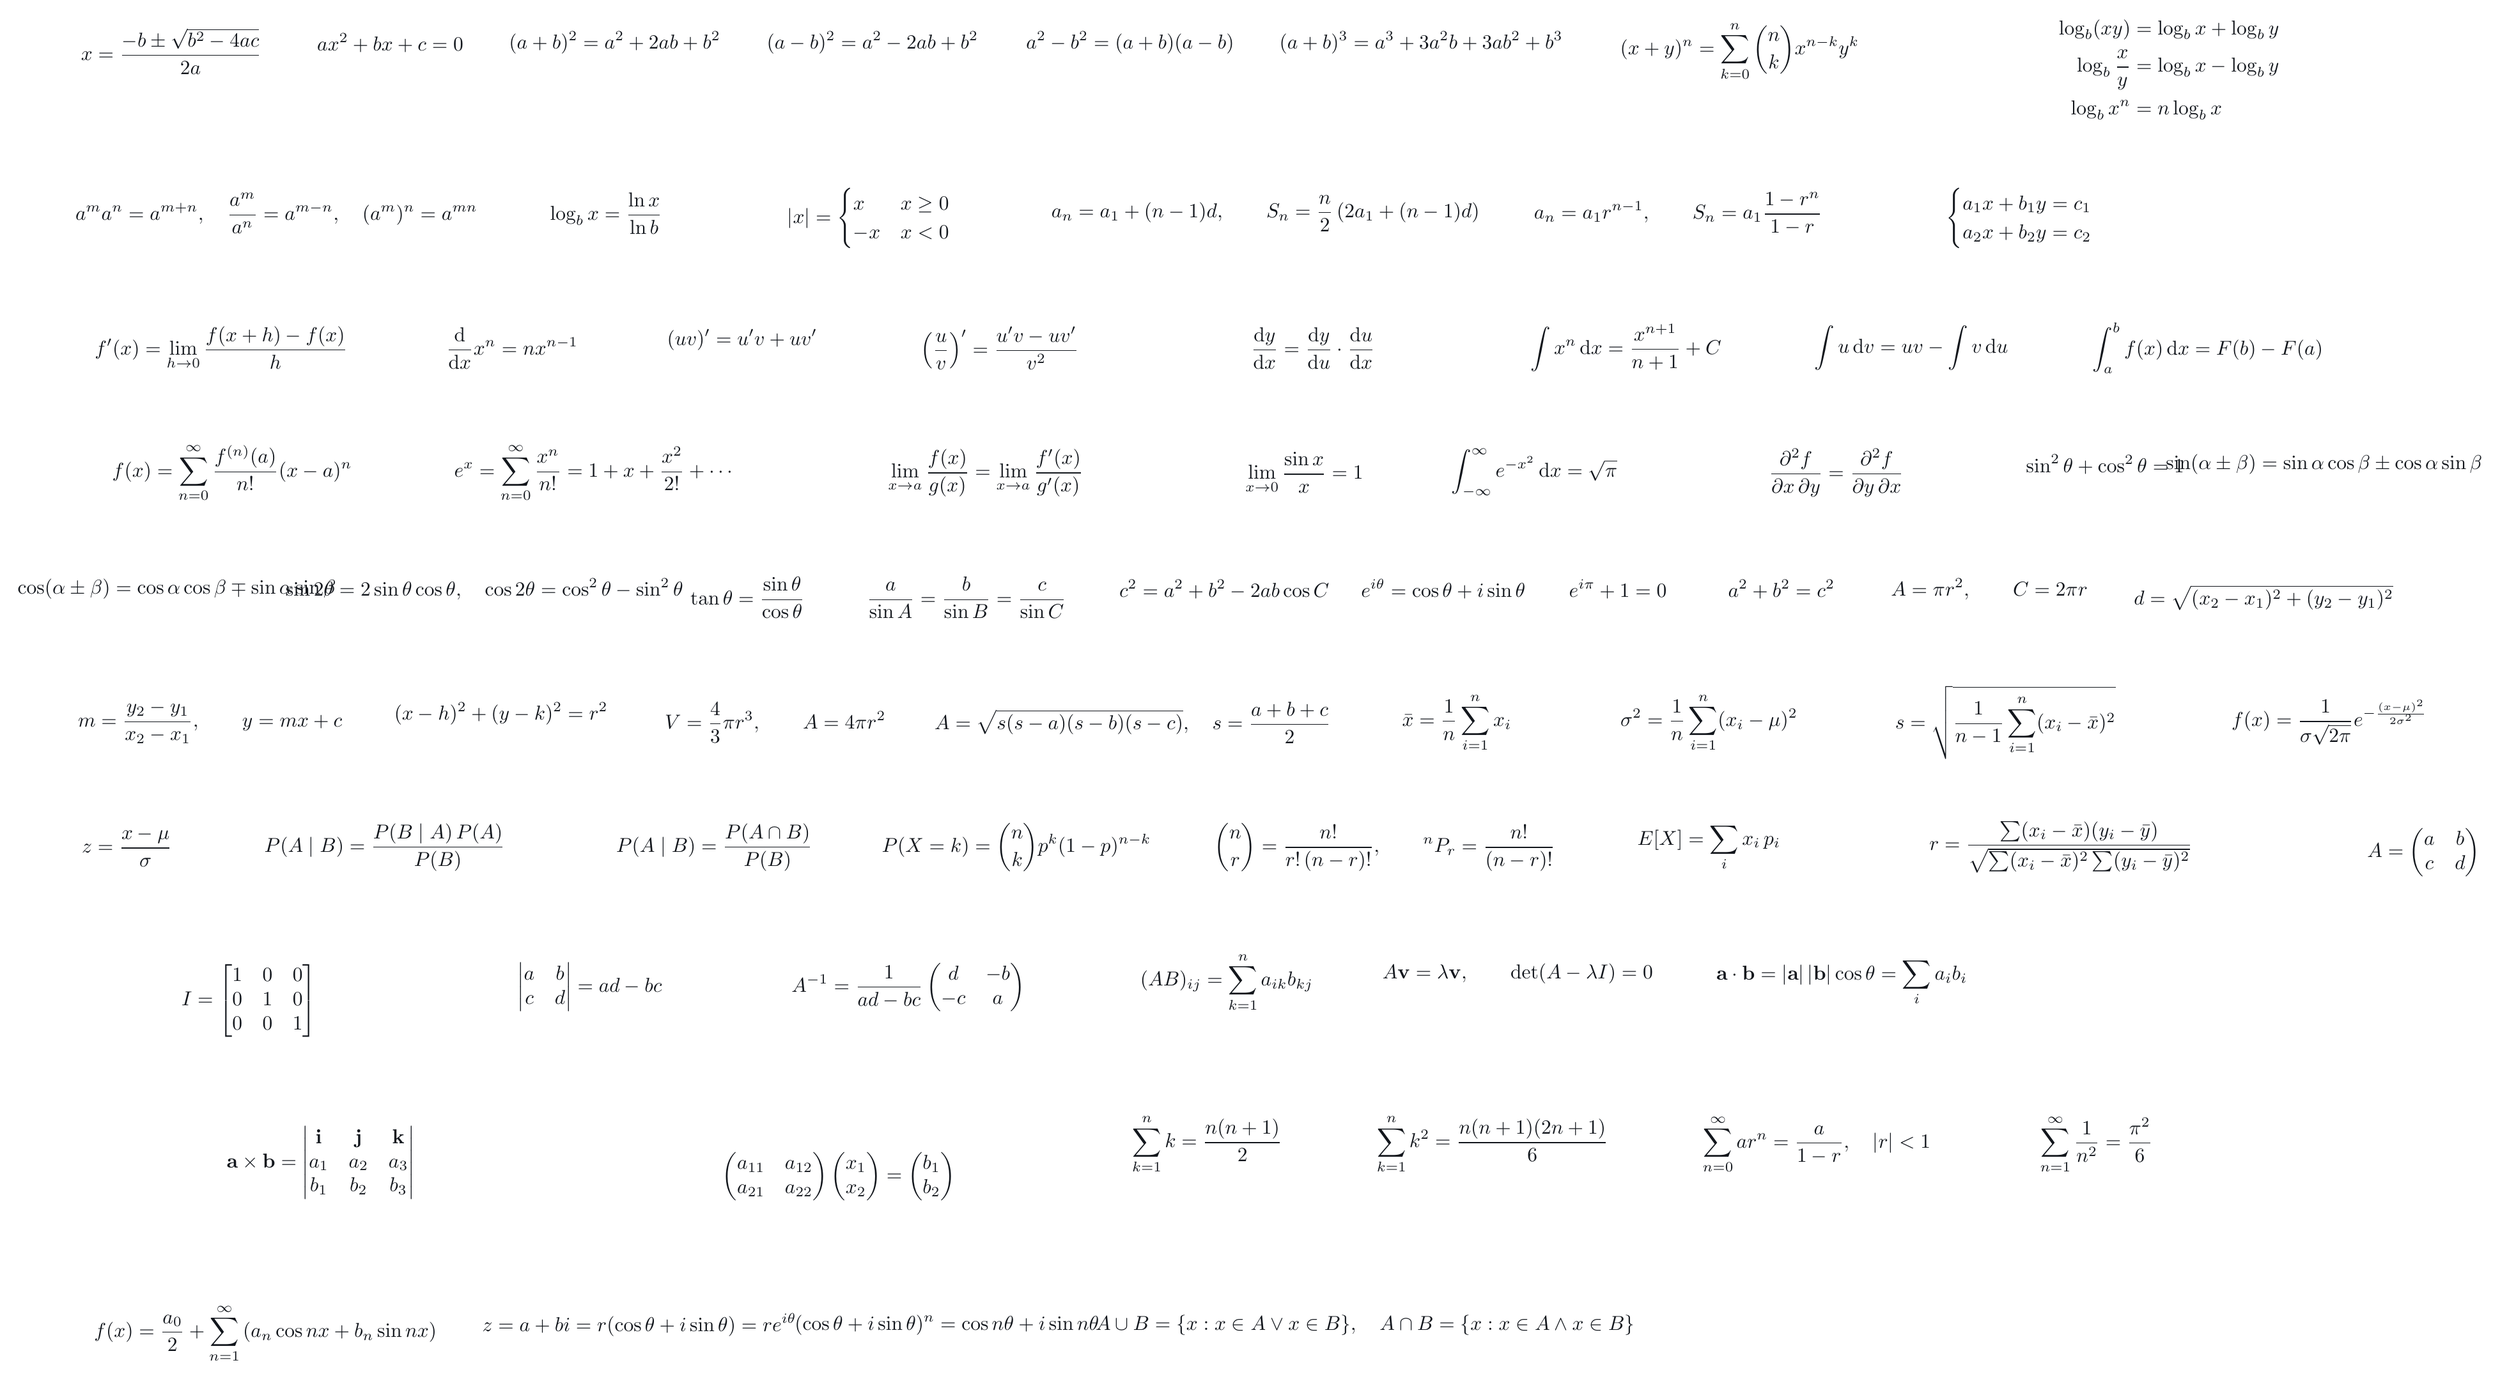
\begin{tikzpicture}[x=1cm, y=1cm]
  % ---- Nodes ----
  % g1 - Formula "x=\frac{-b\pm\sqrt{b^{2}-4ac}}{2a}"
  \node[fcformula, scale=1.138, text=fc12161C]
        (g1) at (3.65,-2.44) {$\displaystyle x=\frac{-b\pm\sqrt{b^{2}-4ac}}{2a}$};
  % g2 - Formula "ax^{2}+bx+c=0"
  \node[fcformula, scale=1.138, text=fc12161C]
        (g2) at (8,-2.27) {$\displaystyle ax^{2}+bx+c=0$};
  % g3 - Formula "(a+b)^{2}=a^{2}+2ab+b^{2}"
  \node[fcformula, scale=1.138, text=fc12161C]
        (g3) at (12.46,-2.27) {$\displaystyle (a+b)^{2}=a^{2}+2ab+b^{2}$};
  % g4 - Formula "(a-b)^{2}=a^{2}-2ab+b^{2}"
  \node[fcformula, scale=1.138, text=fc12161C]
        (g4) at (17.58,-2.27) {$\displaystyle (a-b)^{2}=a^{2}-2ab+b^{2}$};
  % g5 - Formula "a^{2}-b^{2}=(a+b)(a-b)"
  \node[fcformula, scale=1.138, text=fc12161C]
        (g5) at (22.7,-2.27) {$\displaystyle a^{2}-b^{2}=(a+b)(a-b)$};
  % g6 - Formula "(a+b)^{3}=a^{3}+3a^{2}b+3ab^{2}+b^{3}"
  \node[fcformula, scale=1.138, text=fc12161C]
        (g6) at (28.48,-2.27) {$\displaystyle (a+b)^{3}=a^{3}+3a^{2}b+3ab^{2}+b^{3}$};
  % g7 - Formula "(x+y)^{n}=\sum_{k=0}^{n}\binom{n}{k}x^{n-k}y^{k}"
  \node[fcformula, scale=1.138, text=fc12161C]
        (g7) at (34.81,-2.44) {$\displaystyle (x+y)^{n}=\sum_{k=0}^{n}\binom{n}{k}x^{n-k}y^{k}$};
  % g8 - Formula "\begin{aligned} \log_{b}(xy)&=\log_{b}x+\log_{b}"
  \node[fcformula, scale=1.138, text=fc12161C]
        (g8) at (43.34,-2.81) {$\displaystyle \begin{aligned} \log_{b}(xy)&=\log_{b}x+\log_{b}y \\ \log_{b}\frac{x}{y}&=\log_{b}x-\log_{b}y \\ \log_{b}x^{n}&=n\log_{b}x \end{aligned}$};
  % g9 - Formula "a^{m}a^{n}=a^{m+n},\quad \frac{a^{m}}{a^{n}}=a^{"
  \node[fcformula, scale=1.138, text=fc12161C]
        (g9) at (5.74,-5.66) {$\displaystyle a^{m}a^{n}=a^{m+n},\quad \frac{a^{m}}{a^{n}}=a^{m-n},\quad (a^{m})^{n}=a^{mn}$};
  % g10 - Formula "\log_{b}x=\frac{\ln x}{\ln b}"
  \node[fcformula, scale=1.138, text=fc12161C]
        (g10) at (12.29,-5.66) {$\displaystyle \log_{b}x=\frac{\ln x}{\ln b}$};
  % g11 - Formula "|x|=\begin{cases} x & x\geq 0 \\ -x & x<0 \end{c"
  \node[fcformula, scale=1.138, text=fc12161C]
        (g11) at (17.52,-5.76) {$\displaystyle |x|=\begin{cases} x & x\geq 0 \\ -x & x<0 \end{cases}$};
  % g12 - Formula "a_{n}=a_{1}+(n-1)d,\qquad S_{n}=\frac{n}{2}\left"
  \node[fcformula, scale=1.138, text=fc12161C]
        (g12) at (25.39,-5.66) {$\displaystyle a_{n}=a_{1}+(n-1)d,\qquad S_{n}=\frac{n}{2}\left(2a_{1}+(n-1)d\right)$};
  % g13 - Formula "a_{n}=a_{1}r^{n-1},\qquad S_{n}=a_{1}\frac{1-r^{"
  \node[fcformula, scale=1.138, text=fc12161C]
        (g13) at (33.59,-5.66) {$\displaystyle a_{n}=a_{1}r^{n-1},\qquad S_{n}=a_{1}\frac{1-r^{n}}{1-r}$};
  % g14 - Formula "\begin{cases} a_{1}x+b_{1}y=c_{1} \\ a_{2}x+b_{2"
  \node[fcformula, scale=1.138, text=fc12161C]
        (g14) at (40.58,-5.76) {$\displaystyle \begin{cases} a_{1}x+b_{1}y=c_{1} \\ a_{2}x+b_{2}y=c_{2} \end{cases}$};
  % g15 - Formula "f'(x)=\lim_{h\to 0}\frac{f(x+h)-f(x)}{h}"
  \node[fcformula, scale=1.138, text=fc12161C]
        (g15) at (4.64,-8.34) {$\displaystyle f'(x)=\lim_{h\to 0}\frac{f(x+h)-f(x)}{h}$};
  % g16 - Formula "\frac{\mathrm{d}}{\mathrm{d}x}x^{n}=nx^{n-1}"
  \node[fcformula, scale=1.138, text=fc12161C]
        (g16) at (10.42,-8.34) {$\displaystyle \frac{\mathrm{d}}{\mathrm{d}x}x^{n}=nx^{n-1}$};
  % g17 - Formula "(uv)'=u'v+uv'"
  \node[fcformula, scale=1.138, text=fc12161C]
        (g17) at (14.99,-8.17) {$\displaystyle (uv)'=u'v+uv'$};
  % g18 - Formula "\left(\frac{u}{v}\right)'=\frac{u'v-uv'}{v^{2}}"
  \node[fcformula, scale=1.138, text=fc12161C]
        (g18) at (20.11,-8.34) {$\displaystyle \left(\frac{u}{v}\right)'=\frac{u'v-uv'}{v^{2}}$};
  % g19 - Formula "\frac{\mathrm{d}y}{\mathrm{d}x}=\frac{\mathrm{d}"
  \node[fcformula, scale=1.138, text=fc12161C]
        (g19) at (26.33,-8.34) {$\displaystyle \frac{\mathrm{d}y}{\mathrm{d}x}=\frac{\mathrm{d}y}{\mathrm{d}u}\cdot\frac{\mathrm{d}u}{\mathrm{d}x}$};
  % g20 - Formula "\int x^{n}\,\mathrm{d}x=\frac{x^{n+1}}{n+1}+C"
  \node[fcformula, scale=1.138, text=fc12161C]
        (g20) at (32.55,-8.34) {$\displaystyle \int x^{n}\,\mathrm{d}x=\frac{x^{n+1}}{n+1}+C$};
  % g21 - Formula "\int u\,\mathrm{d}v=uv-\int v\,\mathrm{d}u"
  \node[fcformula, scale=1.138, text=fc12161C]
        (g21) at (38.22,-8.34) {$\displaystyle \int u\,\mathrm{d}v=uv-\int v\,\mathrm{d}u$};
  % g22 - Formula "\int_{a}^{b}f(x)\,\mathrm{d}x=F(b)-F(a)"
  \node[fcformula, scale=1.138, text=fc12161C]
        (g22) at (44.11,-8.34) {$\displaystyle \int_{a}^{b}f(x)\,\mathrm{d}x=F(b)-F(a)$};
  % g23 - Formula "f(x)=\sum_{n=0}^{\infty}\frac{f^{(n)}(a)}{n!}(x-"
  \node[fcformula, scale=1.138, text=fc12161C]
        (g23) at (4.86,-10.82) {$\displaystyle f(x)=\sum_{n=0}^{\infty}\frac{f^{(n)}(a)}{n!}(x-a)^{n}$};
  % g24 - Formula "e^{x}=\sum_{n=0}^{\infty}\frac{x^{n}}{n!}=1+x+\f"
  \node[fcformula, scale=1.138, text=fc12161C]
        (g24) at (12.07,-10.82) {$\displaystyle e^{x}=\sum_{n=0}^{\infty}\frac{x^{n}}{n!}=1+x+\frac{x^{2}}{2!}+\cdots$};
  % g25 - Formula "\lim_{x\to a}\frac{f(x)}{g(x)}=\lim_{x\to a}\fra"
  \node[fcformula, scale=1.138, text=fc12161C]
        (g25) at (19.83,-10.82) {$\displaystyle \lim_{x\to a}\frac{f(x)}{g(x)}=\lim_{x\to a}\frac{f'(x)}{g'(x)}$};
  % g26 - Formula "\lim_{x\to 0}\frac{\sin x}{x}=1"
  \node[fcformula, scale=1.138, text=fc12161C]
        (g26) at (26.16,-10.82) {$\displaystyle \lim_{x\to 0}\frac{\sin x}{x}=1$};
  % g27 - Formula "\int_{-\infty}^{\infty}e^{-x^{2}}\,\mathrm{d}x=\"
  \node[fcformula, scale=1.138, text=fc12161C]
        (g27) at (30.73,-10.82) {$\displaystyle \int_{-\infty}^{\infty}e^{-x^{2}}\,\mathrm{d}x=\sqrt{\pi}$};
  % g28 - Formula "\frac{\partial^{2} f}{\partial x\,\partial y}=\f"
  \node[fcformula, scale=1.138, text=fc12161C]
        (g28) at (36.73,-10.82) {$\displaystyle \frac{\partial^{2} f}{\partial x\,\partial y}=\frac{\partial^{2} f}{\partial y\,\partial x}$};
  % g29 - Formula "\sin^{2}\theta+\cos^{2}\theta=1"
  \node[fcformula, scale=1.138, text=fc12161C]
        (g29) at (42.07,-10.65) {$\displaystyle \sin^{2}\theta+\cos^{2}\theta=1$};
  % g30 - Formula "\sin(\alpha\pm\beta)=\sin\alpha\cos\beta\pm\cos\"
  \node[fcformula, scale=1.138, text=fc12161C]
        (g30) at (46.42,-10.65) {$\displaystyle \sin(\alpha\pm\beta)=\sin\alpha\cos\beta\pm\cos\alpha\sin\beta$};
  % g31 - Formula "\cos(\alpha\pm\beta)=\cos\alpha\cos\beta\mp\sin\"
  \node[fcformula, scale=1.138, text=fc12161C]
        (g31) at (3.76,-13.13) {$\displaystyle \cos(\alpha\pm\beta)=\cos\alpha\cos\beta\mp\sin\alpha\sin\beta$};
  % g32 - Formula "\sin 2\theta=2\sin\theta\cos\theta,\quad \cos 2\"
  \node[fcformula, scale=1.138, text=fc12161C]
        (g32) at (9.87,-13.13) {$\displaystyle \sin 2\theta=2\sin\theta\cos\theta,\quad \cos 2\theta=\cos^{2}\theta-\sin^{2}\theta$};
  % g33 - Formula "\tan\theta=\frac{\sin\theta}{\cos\theta}"
  \node[fcformula, scale=1.138, text=fc12161C]
        (g33) at (15.1,-13.3) {$\displaystyle \tan\theta=\frac{\sin\theta}{\cos\theta}$};
  % g34 - Formula "\frac{a}{\sin A}=\frac{b}{\sin B}=\frac{c}{\sin "
  \node[fcformula, scale=1.138, text=fc12161C]
        (g34) at (19.45,-13.3) {$\displaystyle \frac{a}{\sin A}=\frac{b}{\sin B}=\frac{c}{\sin C}$};
  % g35 - Formula "c^{2}=a^{2}+b^{2}-2ab\cos C"
  \node[fcformula, scale=1.138, text=fc12161C]
        (g35) at (24.57,-13.13) {$\displaystyle c^{2}=a^{2}+b^{2}-2ab\cos C$};
  % g36 - Formula "e^{i\theta}=\cos\theta+i\sin\theta"
  \node[fcformula, scale=1.138, text=fc12161C]
        (g36) at (28.92,-13.13) {$\displaystyle e^{i\theta}=\cos\theta+i\sin\theta$};
  % g37 - Formula "e^{i\pi}+1=0"
  \node[fcformula, scale=1.138, text=fc12161C]
        (g37) at (32.39,-13.13) {$\displaystyle e^{i\pi}+1=0$};
  % g38 - Formula "a^{2}+b^{2}=c^{2}"
  \node[fcformula, scale=1.138, text=fc12161C]
        (g38) at (35.64,-13.13) {$\displaystyle a^{2}+b^{2}=c^{2}$};
  % g39 - Formula "A=\pi r^{2},\qquad C=2\pi r"
  \node[fcformula, scale=1.138, text=fc12161C]
        (g39) at (39.77,-13.13) {$\displaystyle A=\pi r^{2},\qquad C=2\pi r$};
  % g40 - Formula "d=\sqrt{(x_{2}-x_{1})^{2}+(y_{2}-y_{1})^{2}}"
  \node[fcformula, scale=1.138, text=fc12161C]
        (g40) at (45.22,-13.3) {$\displaystyle d=\sqrt{(x_{2}-x_{1})^{2}+(y_{2}-y_{1})^{2}}$};
  % g41 - Formula "m=\frac{y_{2}-y_{1}}{x_{2}-x_{1}},\qquad y=mx+c"
  \node[fcformula, scale=1.138, text=fc12161C]
        (g41) at (4.42,-15.78) {$\displaystyle m=\frac{y_{2}-y_{1}}{x_{2}-x_{1}},\qquad y=mx+c$};
  % g42 - Formula "(x-h)^{2}+(y-k)^{2}=r^{2}"
  \node[fcformula, scale=1.138, text=fc12161C]
        (g42) at (10.2,-15.61) {$\displaystyle (x-h)^{2}+(y-k)^{2}=r^{2}$};
  % g43 - Formula "V=\frac{4}{3}\pi r^{3},\qquad A=4\pi r^{2}"
  \node[fcformula, scale=1.138, text=fc12161C]
        (g43) at (15.65,-15.78) {$\displaystyle V=\frac{4}{3}\pi r^{3},\qquad A=4\pi r^{2}$};
  % g44 - Formula "A=\sqrt{s(s-a)(s-b)(s-c)},\quad s=\frac{a+b+c}{2"
  \node[fcformula, scale=1.138, text=fc12161C]
        (g44) at (22.75,-15.78) {$\displaystyle A=\sqrt{s(s-a)(s-b)(s-c)},\quad s=\frac{a+b+c}{2}$};
  % g45 - Formula "\bar{x}=\frac{1}{n}\sum_{i=1}^{n}x_{i}"
  \node[fcformula, scale=1.138, text=fc12161C]
        (g45) at (29.19,-15.78) {$\displaystyle \bar{x}=\frac{1}{n}\sum_{i=1}^{n}x_{i}$};
  % g46 - Formula "\sigma^{2}=\frac{1}{n}\sum_{i=1}^{n}(x_{i}-\mu)^"
  \node[fcformula, scale=1.138, text=fc12161C]
        (g46) at (34.2,-15.78) {$\displaystyle \sigma^{2}=\frac{1}{n}\sum_{i=1}^{n}(x_{i}-\mu)^{2}$};
  % g47 - Formula "s=\sqrt{\frac{1}{n-1}\sum_{i=1}^{n}(x_{i}-\bar{x"
  \node[fcformula, scale=1.138, text=fc12161C]
        (g47) at (40.09,-15.78) {$\displaystyle s=\sqrt{\frac{1}{n-1}\sum_{i=1}^{n}(x_{i}-\bar{x})^{2}}$};
  % g48 - Formula "f(x)=\frac{1}{\sigma\sqrt{2\pi}}e^{-\frac{(x-\mu"
  \node[fcformula, scale=1.138, text=fc12161C]
        (g48) at (46.53,-15.78) {$\displaystyle f(x)=\frac{1}{\sigma\sqrt{2\pi}}e^{-\frac{(x-\mu)^{2}}{2\sigma^{2}}}$};
  % g49 - Formula "z=\frac{x-\mu}{\sigma}"
  \node[fcformula, scale=1.138, text=fc12161C]
        (g49) at (2.77,-18.26) {$\displaystyle z=\frac{x-\mu}{\sigma}$};
  % g50 - Formula "P(A\mid B)=\frac{P(B\mid A)\,P(A)}{P(B)}"
  \node[fcformula, scale=1.138, text=fc12161C]
        (g50) at (7.89,-18.26) {$\displaystyle P(A\mid B)=\frac{P(B\mid A)\,P(A)}{P(B)}$};
  % g51 - Formula "P(A\mid B)=\frac{P(A\cap B)}{P(B)}"
  \node[fcformula, scale=1.138, text=fc12161C]
        (g51) at (14.44,-18.26) {$\displaystyle P(A\mid B)=\frac{P(A\cap B)}{P(B)}$};
  % g52 - Formula "P(X=k)=\binom{n}{k}p^{k}(1-p)^{n-k}"
  \node[fcformula, scale=1.138, text=fc12161C]
        (g52) at (20.44,-18.26) {$\displaystyle P(X=k)=\binom{n}{k}p^{k}(1-p)^{n-k}$};
  % g53 - Formula "\binom{n}{r}=\frac{n!}{r!\,(n-r)!},\qquad {}^{n}"
  \node[fcformula, scale=1.138, text=fc12161C]
        (g53) at (27.76,-18.26) {$\displaystyle \binom{n}{r}=\frac{n!}{r!\,(n-r)!},\qquad {}^{n}P_{r}=\frac{n!}{(n-r)!}$};
  % g54 - Formula "E[X]=\sum_{i}x_{i}\,p_{i}"
  \node[fcformula, scale=1.138, text=fc12161C]
        (g54) at (34.2,-18.26) {$\displaystyle E[X]=\sum_{i}x_{i}\,p_{i}$};
  % g55 - Formula "r=\frac{\sum(x_{i}-\bar{x})(y_{i}-\bar{y})}{\sqr"
  \node[fcformula, scale=1.138, text=fc12161C]
        (g55) at (41.19,-18.26) {$\displaystyle r=\frac{\sum(x_{i}-\bar{x})(y_{i}-\bar{y})}{\sqrt{\sum(x_{i}-\bar{x})^{2}\sum(y_{i}-\bar{y})^{2}}}$};
  % g56 - Formula "A=\begin{pmatrix} a & b \\ c & d \end{pmatrix}"
  \node[fcformula, scale=1.138, text=fc12161C]
        (g56) at (48.4,-18.36) {$\displaystyle A=\begin{pmatrix} a & b \\ c & d \end{pmatrix}$};
  % g57 - Formula "I=\begin{bmatrix} 1 & 0 & 0 \\ 0 & 1 & 0 \\ 0 & "
  \node[fcformula, scale=1.138, text=fc12161C]
        (g57) at (5.19,-21.31) {$\displaystyle I=\begin{bmatrix} 1 & 0 & 0 \\ 0 & 1 & 0 \\ 0 & 0 & 1 \end{bmatrix}$};
  % g58 - Formula "\begin{vmatrix} a & b \\ c & d \end{vmatrix}=ad-"
  \node[fcformula, scale=1.138, text=fc12161C]
        (g58) at (11.96,-21.04) {$\displaystyle \begin{vmatrix} a & b \\ c & d \end{vmatrix}=ad-bc$};
  % g59 - Formula "A^{-1}=\frac{1}{ad-bc}\begin{pmatrix} d & -b \\ "
  \node[fcformula, scale=1.138, text=fc12161C]
        (g59) at (18.29,-21.04) {$\displaystyle A^{-1}=\frac{1}{ad-bc}\begin{pmatrix} d & -b \\ -c & a \end{pmatrix}$};
  % g60 - Formula "(AB)_{ij}=\sum_{k=1}^{n}a_{ik}b_{kj}"
  \node[fcformula, scale=1.138, text=fc12161C]
        (g60) at (24.62,-20.94) {$\displaystyle (AB)_{ij}=\sum_{k=1}^{n}a_{ik}b_{kj}$};
  % g61 - Formula "A\mathbf{v}=\lambda\mathbf{v},\qquad \det(A-\lam"
  \node[fcformula, scale=1.138, text=fc12161C]
        (g61) at (30.4,-20.77) {$\displaystyle A\mathbf{v}=\lambda\mathbf{v},\qquad \det(A-\lambda I)=0$};
  % g62 - Formula "\mathbf{a}\cdot\mathbf{b}=|\mathbf{a}|\,|\mathbf"
  \node[fcformula, scale=1.138, text=fc12161C]
        (g62) at (36.84,-20.94) {$\displaystyle \mathbf{a}\cdot\mathbf{b}=|\mathbf{a}|\,|\mathbf{b}|\cos\theta=\sum_{i}a_{i}b_{i}$};
  % g63 - Formula "\mathbf{a}\times\mathbf{b}=\begin{vmatrix} \math"
  \node[fcformula, scale=1.138, text=fc12161C]
        (g63) at (6.62,-24.53) {$\displaystyle \mathbf{a}\times\mathbf{b}=\begin{vmatrix} \mathbf{i} & \mathbf{j} & \mathbf{k} \\ a_{1} & a_{2} & a_{3} \\ b_{1} & b_{2} & b_{3} \end{vmatrix}$};
  % g64 - Formula "\begin{pmatrix} a_{11} & a_{12} \\ a_{21} & a_{2"
  \node[fcformula, scale=1.138, text=fc12161C]
        (g64) at (16.91,-24.8) {$\displaystyle \begin{pmatrix} a_{11} & a_{12} \\ a_{21} & a_{22} \end{pmatrix}\begin{pmatrix} x_{1} \\ x_{2} \end{pmatrix}=\begin{pmatrix} b_{1} \\ b_{2} \end{pmatrix}$};
  % g65 - Formula "\sum_{k=1}^{n}k=\frac{n(n+1)}{2}"
  \node[fcformula, scale=1.138, text=fc12161C]
        (g65) at (24.23,-24.16) {$\displaystyle \sum_{k=1}^{n}k=\frac{n(n+1)}{2}$};
  % g66 - Formula "\sum_{k=1}^{n}k^{2}=\frac{n(n+1)(2n+1)}{6}"
  \node[fcformula, scale=1.138, text=fc12161C]
        (g66) at (29.9,-24.16) {$\displaystyle \sum_{k=1}^{n}k^{2}=\frac{n(n+1)(2n+1)}{6}$};
  % g67 - Formula "\sum_{n=0}^{\infty}ar^{n}=\frac{a}{1-r},\quad |r"
  \node[fcformula, scale=1.138, text=fc12161C]
        (g67) at (36.34,-24.16) {$\displaystyle \sum_{n=0}^{\infty}ar^{n}=\frac{a}{1-r},\quad |r|<1$};
  % g68 - Formula "\sum_{n=1}^{\infty}\frac{1}{n^{2}}=\frac{\pi^{2}"
  \node[fcformula, scale=1.138, text=fc12161C]
        (g68) at (41.9,-24.16) {$\displaystyle \sum_{n=1}^{\infty}\frac{1}{n^{2}}=\frac{\pi^{2}}{6}$};
  % g69 - Formula "f(x)=\frac{a_{0}}{2}+\sum_{n=1}^{\infty}\left(a_"
  \node[fcformula, scale=1.138, text=fc12161C]
        (g69) at (5.52,-27.92) {$\displaystyle f(x)=\frac{a_{0}}{2}+\sum_{n=1}^{\infty}\left(a_{n}\cos nx+b_{n}\sin nx\right)$};
  % g70 - Formula "z=a+bi=r(\cos\theta+i\sin\theta)=re^{i\theta}"
  \node[fcformula, scale=1.138, text=fc12161C]
        (g70) at (12.95,-27.75) {$\displaystyle z=a+bi=r(\cos\theta+i\sin\theta)=re^{i\theta}$};
  % g71 - Formula "(\cos\theta+i\sin\theta)^{n}=\cos n\theta+i\sin "
  \node[fcformula, scale=1.138, text=fc12161C]
        (g71) at (19.06,-27.75) {$\displaystyle (\cos\theta+i\sin\theta)^{n}=\cos n\theta+i\sin n\theta$};
  % g72 - Formula "A\cup B=\{x : x\in A\lor x\in B\},\quad A\cap B="
  \node[fcformula, scale=1.138, text=fc12161C]
        (g72) at (27.37,-27.75) {$\displaystyle A\cup B=\{x : x\in A\lor x\in B\},\quad A\cap B=\{x : x\in A\land x\in B\}$};
\end{tikzpicture}
\end{document}